\documentclass[
	a4paper,
	11pt
]
{article}

%%% Font packages

\usepackage[LGR,T1]{fontenc}
\usepackage[utf8]{inputenc}
\usepackage{lmodern}
\usepackage{microtype}
\usepackage{upgreek}
\usepackage[misc]{ifsym}

%%% Maths and science packages

\usepackage{amsmath,amsthm,amssymb}
\usepackage{pgfplots}
	\usetikzlibrary{
		calc,
		patterns,
		positioning
	}
	\pgfplotsset{
		compat=1.16,
		samples=200,
		clip=false,
		my axis style/.style={
			axis x line=middle,
			axis y line=middle,
			legend pos=outer north east,
			axis line style={
				->,
			},
			legend style={
				font=\footnotesize
			},
			label style={
				font=\footnotesize
			},
			tick label style={
				font=\footnotesize
			},
			xlabel style={
				at={
					(ticklabel* cs:1)
				},
				anchor=west,
				font=\footnotesize,
			},
			ylabel style={
				at={
					(ticklabel* cs:1)
				},
				anchor=west,
				font=\footnotesize,
			},
			xlabel=$X$,
			ylabel=$Y$
		},
	}
	\tikzset{
		>=stealth
	}

%%% Tables and figures packages

\usepackage{float}
\usepackage{caption}
	\captionsetup{
		format=plain,
		labelfont=bf,
		font=small,
		justification=centering
	}
	
%%% Numbers and sets

\newcommand{\E}{\mathrm{e}}

%%% Title, author, date

\title{Using the \texttt{tikzpicture} Environment for Drawing Graphs in \LaTeX}
\author{Bob Jones}
\date{\today}

\begin{document}

\maketitle

My awesome graph is shown in Figure~\ref{fig:my-awesome-graph}.

\begin{figure}[h]
	\centering
	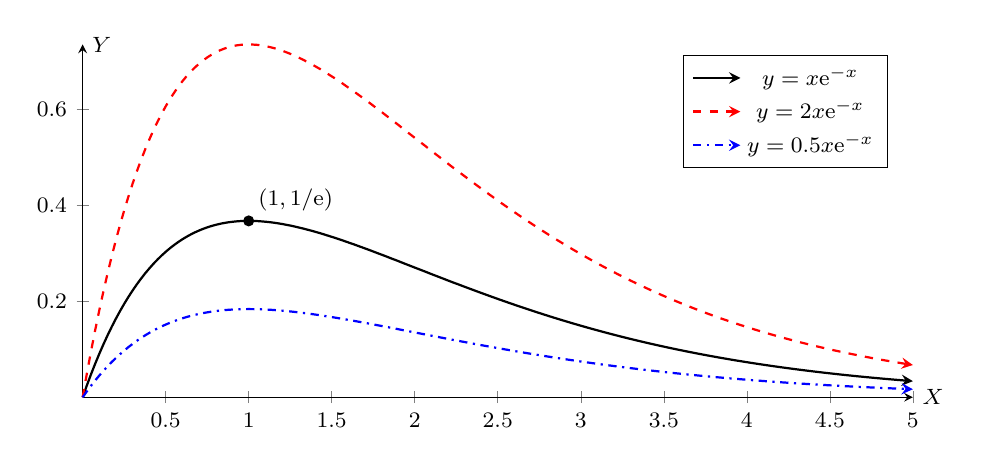
\begin{tikzpicture}
	\begin{axis}[
		my axis style,
		width=\textwidth,
		height=.5\textwidth,
		legend entries={
			$y = x\E^{-x}$,
			$y = 2x\E^{-x}$,
			$y = 0.5x\E^{-x}$
		},
		legend pos=north east
	]
	
	\addplot[
		domain=0:5,
		thick,
		->
	]
	{x*exp(-x)};

	\addplot[
		domain=0:5,
		thick,
		red,
		dashed,
		->
	]
	{2*x*exp(-x)};

	\addplot[
		domain=0:5,
		thick,
		blue,
		dashdotted,
		->
	]
	{.5*x*exp(-x)};
	
	\fill[
		black
	]
	(1,.36788) circle (2pt) node[above right] {\footnotesize $(1, 1/\E)$};
	
	\end{axis}
	\end{tikzpicture}
	\caption{My awesome graph.}
	\label{fig:my-awesome-graph}
\end{figure}

\end{document}